% 
% topic Template for ME3023 - Measurements in Mechanincal Systems - Tennessee Technological University
%
% Spring 2020 - Summer 2020
% Tristan Hill, May 31, 2020
% Introduction - Topic 1 - General Measurement System
%

\documentclass{beamer}                         % for presentation (has nav buttons at bottom)
%\documentclass[handout]{beamer}  % for handout 
\usepackage{beamerthemesplit}
\usepackage{amsmath}
\usepackage{listings}
\usepackage{multicol}
\usepackage{framed}

\beamertemplateballitem

\definecolor{TTUpurple}{rgb}{0.3098, 0.1607, 0.5176} % TTU Purple (primary)
\definecolor{TTUgold}{rgb}{1.0000, 0.8666, 0.0000} % TTU Gold (primary)

\setbeamercolor{palette primary}{bg=TTUpurple,fg=TTUgold}
\setbeamercolor{palette secondary}{bg=black,fg=TTUgold}
\setbeamercolor{palette tertiary}{bg=black,fg=TTUpurple}
\setbeamercolor{palette quaternary}{bg=TTUgold,fg=black}
\setbeamercolor{structure}{fg=TTUpurple} % itemize, enumerate, etc
\setbeamercolor{section in toc}{fg=TTUpurple} % TOC sections

% custom colors 
\definecolor{mygray}{rgb}{.6, .6, .6}
\definecolor{mypurple}{rgb}{0.6,0.1961,0.8}
\definecolor{mybrown}{rgb}{0.5451,0.2706,0.0745}
\definecolor{mygreen}{rgb}{0, .39, 0}

% color commands
\newcommand{\R}{\color{red}}
\newcommand{\B}{\color{blue}}
\newcommand{\BR}{\color{mybrown}}
\newcommand{\K}{\color{black}}
\newcommand{\G}{\color{mygreen}}
\newcommand{\PR}{\color{mypurple}}
%\usefonttheme{professionalfonts}

\newcommand{\Lagr}{\mathcal{L}} % lagrangian

\newcommand{\vspccc}{\vspace{6mm}\\} % large vertical space
\newcommand{\vspcc}{\vspace{4mm}\\}   % medium vertical space
\newcommand{\vspc}{\vspace{2mm}\\}     % small vertical space

\newcommand{\hspcccc}{\hspace{10mm}} % large horizontal space
\newcommand{\hspccc}{\hspace{6mm}} % large horizontal space
\newcommand{\hspcc}{\hspace{4mm}}   % medium horizontal space
\newcommand{\hspc}{\hspace{2mm}}     % small horizontal space


\author{ME3023 - Measurements in Mechanical Systems} % original formatting from Mike Renfro, September 21, 2004

\newcommand{\MNUM}{1\hspace{2mm}} % Module number
\newcommand{\TNUM}{1\hspace{2mm}} % Topic number 
\newcommand{\moduletitle}{Introduction }
\newcommand{\topictitle}{General Measurement System } 

\title{Module \MNUM - \moduletitle}

\date{Mechanical Engineering\\Tennessee Technological University}

\begin{document}

\lstset{language=MATLAB,basicstyle=\ttfamily\small,showstringspaces=false}

\frame{\titlepage \center\begin{framed}\Large \textbf{Topic \TNUM - \topictitle}\end{framed} \vspace{5mm}}

% Section 0: Outline

\frame{

\large \textbf{Topic \TNUM - \topictitle} \vspace{3mm}\\

\begin{itemize}
	\item Welcome Back!\vspace{3mm}\\ % Section 1
	\item Definition of a Measurement\vspace{3mm}\\% Section 2
	\item Measurement System Stages\vspace{3mm}\\ %Section 3
	\item Examples in Mechanical Engineering \vspace{3mm}\\ %Section 4

	%\item Example\vspace{3mm}\\ % Section 5 - 5 is almost too many...
\end{itemize}
}

% Section 1
\section{Welcome Back!}

\frame{
\frametitle{Welcome to New Video Topics}
\large{\it Welcome Back!\vspace{3mm}\\}

\begin{itemize}
\item Things are going to be different but we will still learn! \vspace{3mm}\\
\item These new outlines should help keep me/us on track.  \vspace{3mm}\\
\item The material will be organized in $\sim 10$ min videos, and you can watch them at anytime. \vspace{3mm}\\
\end{itemize}

}

% Section 2
\section{Definition of a Measurement}

\frame{
\frametitle{Definition of a Measurement}

\large{``A {\bf \B measurement} is an act of assigning a specific value to a physical variable.''} \vspc
{\tiny Text: Theory and Design of Mech. Meas.}

}

% Section 3
\section{Measurement System Stages}

\frame{
\frametitle{Measurement System Stages}

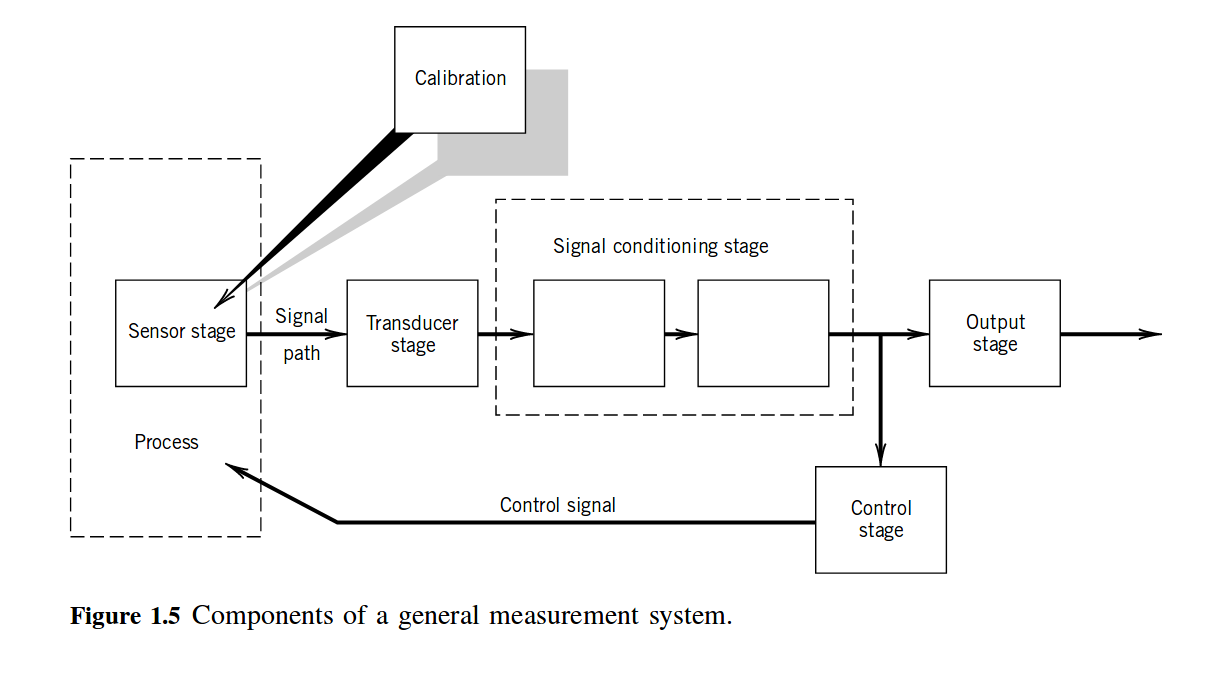
\includegraphics[scale=.3]{measurement_stages} \\
{\tiny Image: Theory and Design of Mech. Meas.}
}

\frame{
\frametitle{Sensor-Transducer Stage}
a {\PR sensor}, a physical element that employs some natural phenomenon... ...to sense the variable being measured
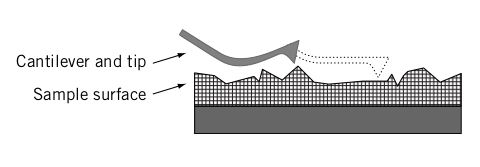
\includegraphics[scale=0.20]{sensor_stage.png}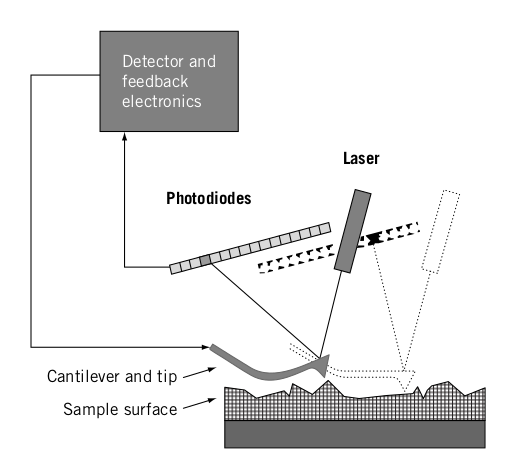
\includegraphics[scale=0.20]{sensor_transducer_stage}\\

A {\G transducer} converts the sensed information into a detectable signal \\
{\tiny Text, Image: Theory and Design of Mech. Meas.}
}

\frame{
\frametitle{Signal Conditioning Stage}

What is the the definition of {\B signal}? \vspc

\begin{multicols}{2}
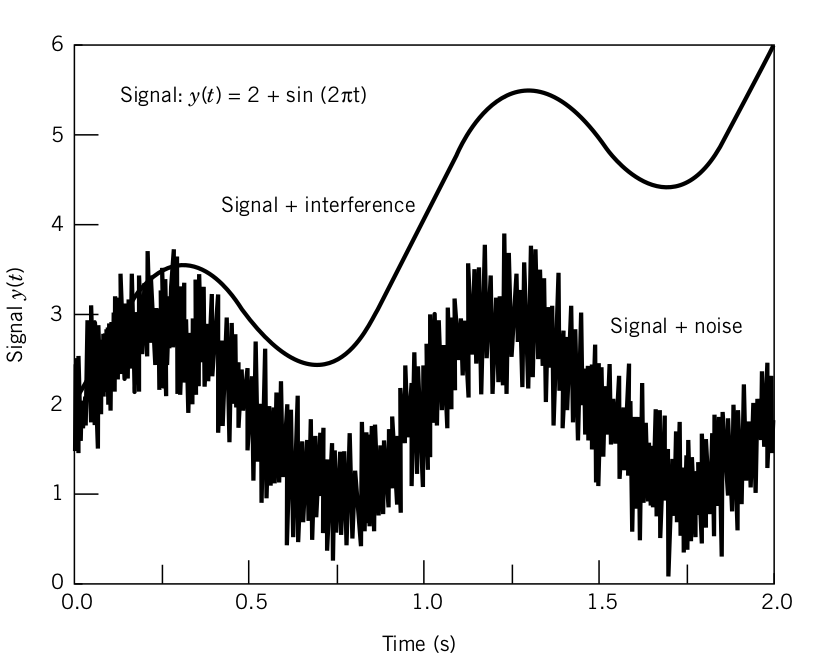
\includegraphics[scale=0.18]{signal_noise.png}

\begin{itemize}
\item Filtering
\item Amplification
\item Attenuation
\item Excitation 
\item Linearization
\item Electrical Isolation
\item Surge Protection
\end{itemize}

\end{multicols}

{\tiny Image: Theory and Design of Mech. Meas.}
}

\frame{
\frametitle{Output Stage}
The {\BR output stage} indicates or records the value measured. This might be a simple readout
display, a marked scale, or even a recording device such as a computer disk drive.

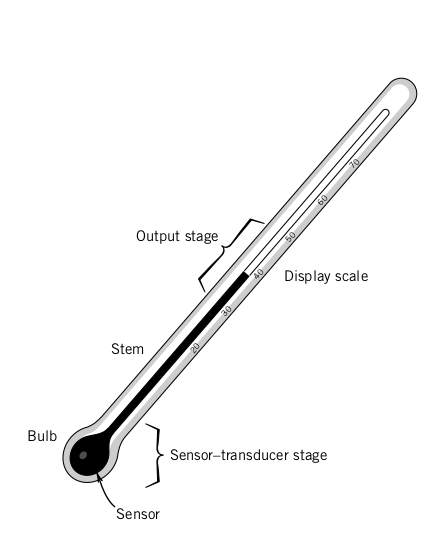
\includegraphics[scale=0.25]{bulb_thermometer.png} \hspace{10mm}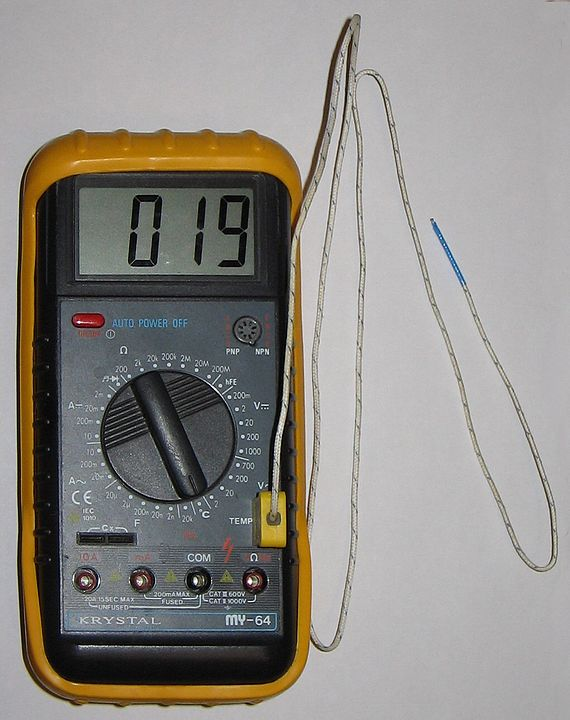
\includegraphics[scale=0.3]{thermocouple.jpg}

{\tiny Image: Theory and Design of Mech. Meas. \hspace{20mm} Image: \href{https://en.wikipedia.org/wiki/Thermocouple}{Wikipedia} }
}

% Section 4
\section{Engineering Example}

\frame{
\frametitle{Engineering Example}

\begin{multicols}{2}
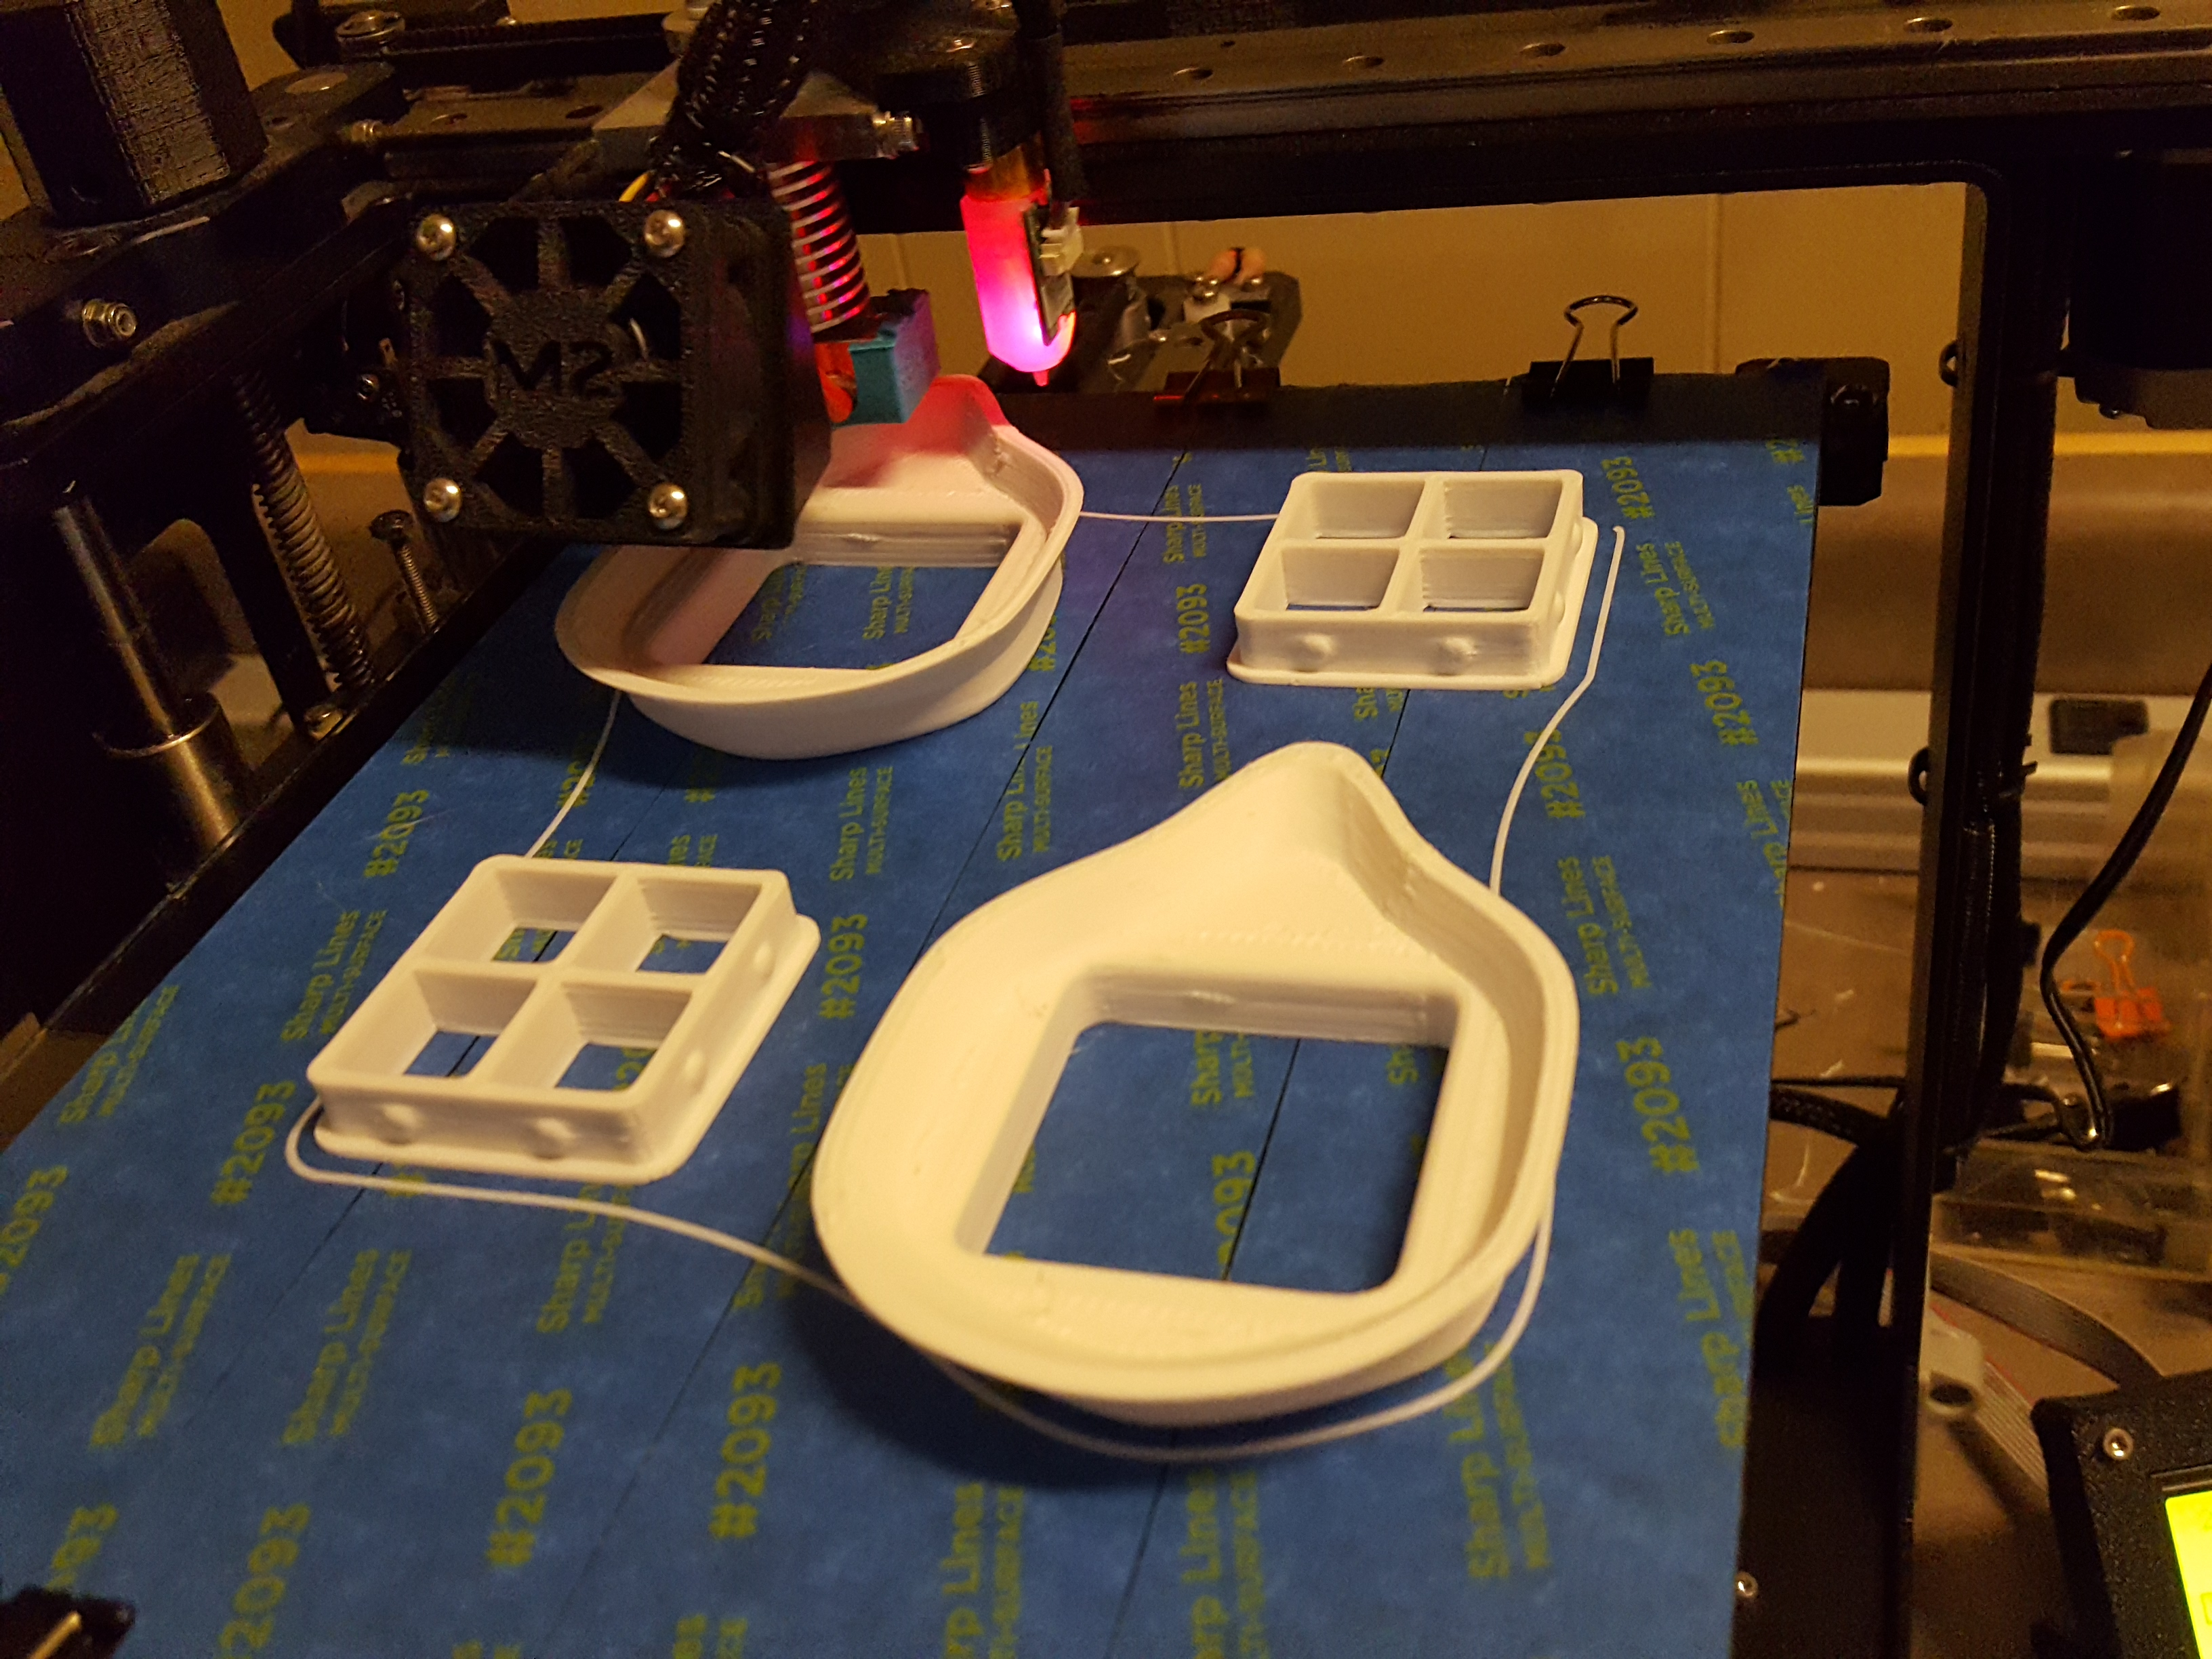
\includegraphics[scale=0.04]{makethemask.jpg}

\small
3D printers (FDM) use PLA, ABS, PETG and other plastics which absorb moisture from the air over time causing adverse affects on part quality. This is particularly a problem in humid climates such the southeastern USA.
\end{multicols}

{\tiny Image: T.Hill}

}

\frame{
\frametitle{Engineering Example}

\begin{multicols}{2}

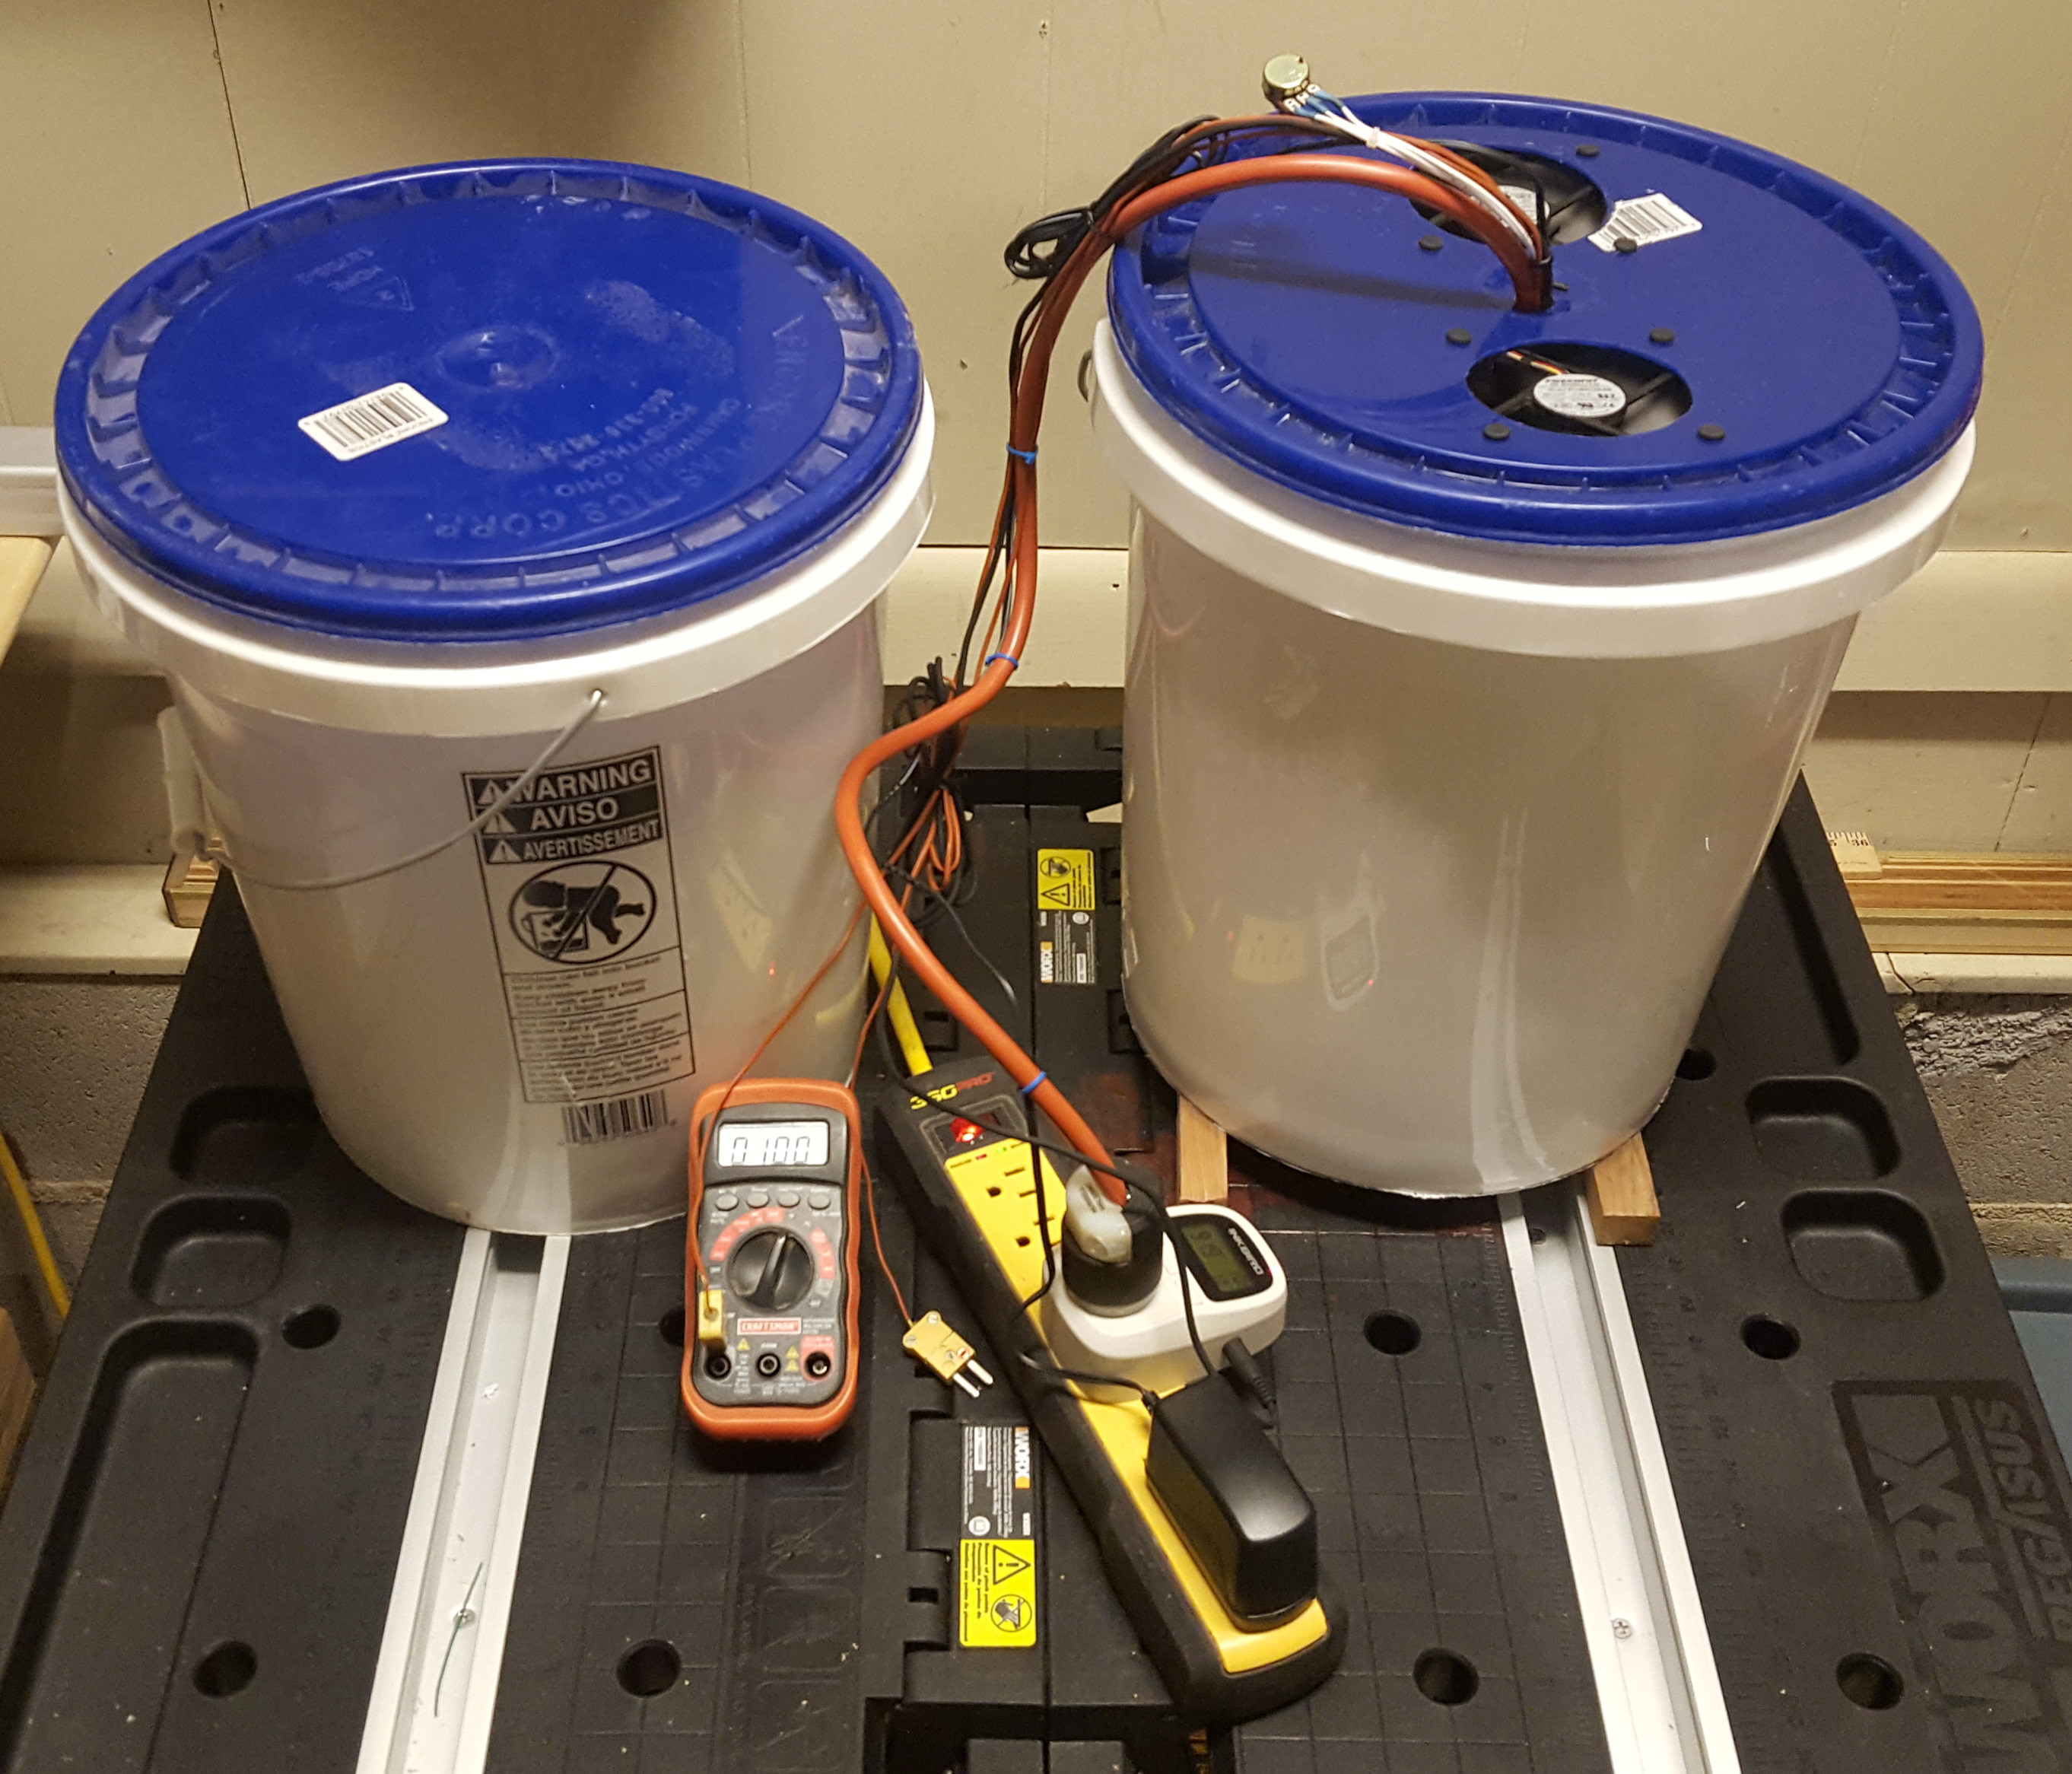
\includegraphics[scale=0.055]{filament_dryer_fig2.jpg}


\small
\vspace{10mm}Fortunately the {\it water-logged} plastic can be dehydrated for further use.\vspcc
Inspect the DIY filament dryer shown and Identify each of the following measurement stages.

\begin{itemize}
\item Sensor - Transducer
\item Signal Condtioning
\item Output Stage
\item Feedback Control ?
\end{itemize}

\end{multicols}

{\tiny Image: T.Hill}
}

\end{document}





